%% LaTeX-Beamer template for KIT design
%% by Erik Burger, Christian Hammer
%% title picture by Klaus Krogmann
%%
%% version 2.1
%%
%% mostly compatible to KIT corporate design v2.0
%% http://intranet.kit.edu/gestaltungsrichtlinien.php
%%
%% Problems, bugs and comments to
%% burger@kit.edu

\documentclass[18pt]{beamer}
\usepackage[utf8]{inputenc}
\usepackage[T1]{fontenc}
\usepackage{microtype}
%% SLIDE FORMAT

% use 'beamerthemekit' for standard 4:3 ratio
% for widescreen slides (16:9), use 'beamerthemekitwide'

\usepackage{templates/beamerthemekit}
% \usepackage{templates/beamerthemekitwide}
\usepackage{amsmath}
\usepackage{amsfonts}
\usepackage{amssymb}
\usepackage{siunitx}
\sisetup{range-units = single, range-phrase = {-}, separate-uncertainty = true,multi-part-units=brackets, product-units=brackets, locale=US, detect-weight=true, binary-units=true}
\usepackage{color}
\usepackage{todonotes}
\presetkeys{todonotes}{inline}{}
\usepackage{booktabs}
\usepackage{listings}
\usepackage{parnotes}
\usepackage{xspace}
\usepackage{multirow}
\usepackage{multicol}
\usepackage{subfig}
\usepackage{caption}
\captionsetup{font=scriptsize,labelfont=scriptsize}

\usepackage{chngcntr}
\counterwithin{figure}{section}
\counterwithin{table}{section}
\setbeamertemplate{caption}[numbered]

% settings for making the table of contents less ugly
\setbeamertemplate{section in toc}{\inserttocsectionnumber\ \ ~\inserttocsection}
\setbeamertemplate{subsection in toc}{\qquad\inserttocsectionnumber.\inserttocsubsectionnumber\ \ ~\inserttocsubsection\\ }

% bibliography
%\usepackage[style=numeric, backend=biber, sorting=ynt]{biblatex}
%\addbibresource{bibliography.bib}
\beamertemplatenavigationsymbolsempty
%% TITLE PICTURE

% if a custom picture is to be used on the title page, copy it into the 'logos'
% directory, in the line below, replace 'mypicture' with the 
% filename (without extension) and uncomment the following line
% (picture proportions: 63 : 20 for standard, 169 : 40 for wide
% *.eps format if you use latex+dvips+ps2pdf, 
% *.jpg/*.png/*.pdf if you use pdflatex)

%\titleimage{Karlsruher_Schloss_Front_Panorama}


%% TITLE LOGO

% for a custom logo on the front page, copy your file into the 'logos'
% directory, insert the filename in the line below and uncomment it

\titlelogo{nologo.png}

% (*.eps format if you use latex+dvips+ps2pdf,
% *.jpg/*.png/*.pdf if you use pdflatex)

%% TikZ INTEGRATION

% use these packages for PCM symbols and UML classes
% \usepackage{templates/tikzkit}
% \usepackage{templates/tikzuml}

% Define KIT Colors
\definecolor{KIT-Gruen}{RGB}{0,150,130}
\definecolor{KIT-Blau}{RGB}{70,100,170}
\definecolor{KIT-MaiGruen}{RGB}{140,182,60}
\definecolor{KIT-Gelb}{RGB}{252,229,0}
\definecolor{KIT-Orange}{RGB}{223,155,27}
\definecolor{KIT-Braun}{RGB}{167,130,46}
\definecolor{KIT-Rot}{RGB}{162,34,35}
\definecolor{KIT-Lila}{RGB}{163,16,124}
\definecolor{KIT-Cyan-Blau}{RGB}{35,161,224}


% Define some commands
% arrows
\newcommand{\rar}{\ensuremath{\rightarrow}\xspace}
\newcommand{\Rar}{\ensuremath{\Rightarrow}\xspace}

% particle physics
\newcommand{\ttbar}{\text{t}$\overline{\text{t}}$\xspace }
\newcommand{\boldttbar}{\textbf{t}$\overline{\textbf{t}}$\xspace}
\newcommand{\ttbarH}{\text{t}$\overline{\text{t}}$H\xspace }
\newcommand{\boldttbarH}{\textbf{t}$\overline{\textbf{t}}$\textbf{H}\xspace}
\newcommand{\bbbar}{\text{b}$\overline{\text{b}}$\xspace }
\newcommand{\ccbar}{\text{c}$\overline{\text{c}}$\xspace }
\newcommand{\pT}{${p_{T}}$\xspace}
\newcommand{\Htobb}{H$\to $ \bbbar}

\newcommand{\pathToPlots}{plots}
\newcommand{\pathToTables}{tables}

\newcommand{\catname}{jge6_t3}
\newcommand{\frameCatName}{63}
\newcommand{\scaledProcessName}{63445464_ttHbb_N1000_ttbarOther_0p9}
\newcommand{\frameScaledProcessName}{$\ttbar\cdot 0.9$}

\newcommand{\createFrameSet}[2]{
\begin{frame}{\frameCatName - #1 PostfitB}
\vskip -0.5cm
\begin{figure}
\centering
\subfloat[Normalization Distribution]{\includegraphics[width=.4\textwidth]{plots/ljets_\catname_normalisation_#2_PostfitB.pdf}}
\subfloat[Mean And Median Values of Distributions]{\includegraphics[width=.4\textwidth]{plots/ljets_\catname_normalisation_#2_mean_PostfitB.pdf}}
\caption[PostfitB Normalization Distribution for #1 in category \frameCatName with $\num{1.5}\cdot$ \ttbar\bbbar]{PostfitB Normalization Distribution for #1 in category \frameCatName with $\num{1.5}\cdot$ \ttbar\bbbar. Each histogram ($\mu=0$ and $\mu=1$) contains at least 900 toys, respectively.}
\end{figure}
\end{frame}

\begin{frame}{\frameCatName - #1 PostfitS}
\begin{figure}
\subfloat[Normalization Distribution PostfitS]{\includegraphics[width=.4\textwidth]{plots/ljets_\catname_normalisation_#2_PostfitS.pdf}}
\subfloat[Mean And Median Values of Distributions PostfitS]{\includegraphics[width=.4\textwidth]{plots/ljets_\catname_normalisation_#2_mean_PostfitS.pdf}}
\caption[PostfitS Normalization Distribution for #1 in category \frameCatName with $\num{1.5}\cdot$ \ttbar\bbbar]{PostfitS Normalization Distribution for #1 in category \frameCatName with $\num{1.5}\cdot$ \ttbar\bbbar. Each histogram ($\mu=0$ and $\mu=1$) contains at least 900 toys, respectively.}
\end{figure}
\end{frame}
}

\newcommand{\createNormTableFrame}[6]{

\begin{frame}{Normalization for #3 - #1 - Values for $\mu = #5$}
\begin{scriptsize}
\input{tables/63445464_ttHbb_N1000_#2_ljets_#4_normalisation_values_nominal_S_#6}
\end{scriptsize}

\end{frame}
}
\newcommand{\createPullplotFrame}[4]{
\begin{frame}{#1 - #3 - Pullplots}
\vskip -0.75cm
\begin{figure}
\centering
\subfloat[Pull Plot for $\mu = 0$]{\includegraphics[width=.5\textwidth]{plots/63445464_ttHbb_N1000_#2_ljets_#4_normalisation_pullplot_nominal_S_0p0.pdf}}
\subfloat[Pull Plot for $\mu = 1$]{\includegraphics[width=.5\textwidth]{plots/63445464_ttHbb_N1000_#2_ljets_#4_normalisation_pullplot_nominal_S_1p0.pdf}}
\caption[Normalization Pull Plots for Category #3 with #1]{Normalization Pull Plots for Category #3 with #1 for a background-only (blue) and a signal+background (red) fit.  Circles are mean values of the respective process normalization distribution, squares the median. All values were normed to the respective prefit values. The dotted red line shows the expected values.}
\end{figure}
\end{frame}
}
\newcommand{\createNormFrameSet}[2]{

\createPullplotFrame{#1}{#2}{44}{j4_t4}
\createNormTableFrame{#1}{#2}{44}{j4_t4}{0.0}{0p0}
\createNormTableFrame{#1}{#2}{44}{j4_t4}{1.0}{1p0}

\createPullplotFrame{#1}{#2}{54}{j5_tge4}
\createNormTableFrame{#1}{#2}{54}{j5_tge4}{0.0}{0p0}
\createNormTableFrame{#1}{#2}{54}{j5_tge4}{1.0}{1p0}

\createPullplotFrame{#1}{#2}{63}{jge6_t3}
\createNormTableFrame{#1}{#2}{63}{jge6_t3}{0.0}{0p0}
\createNormTableFrame{#1}{#2}{63}{jge6_t3}{1.0}{1p0}

\createPullplotFrame{#1}{#2}{64}{jge6_tge4}
\createNormTableFrame{#1}{#2}{64}{jge6_tge4}{0.0}{0p0}
\createNormTableFrame{#1}{#2}{64}{jge6_tge4}{1.0}{1p0}

}





% the presentation starts here

\title[JES uncertainty study]{JES uncertainty study}
%\subtitle{Status Update}
\author[Philip Keicher]{Karim~El~Morabit, Matthias~Schröder, \textbf{Philip Keicher}}

\institute{Institut für Experimentelle Kernphysik (IEKP)}
%\date{June 29th 2017}

\begin{document}

% change the following line to "ngerman" for German style date and logos
%\selectlanguage{ngerman}
\selectlanguage{english}


%title page
\begin{frame}
\titlepage
\end{frame}

\section*{Outline}
%\subsection*{Outline}
\begin{frame}[label={outline}]
	\frametitle{Outline}
	\tableofcontents
\end{frame}


\section{Motivation}
%\subsection{Subsection 1.1}
\begin{frame}{Motivation}
\begin{figure}
\centering

\includegraphics[scale = 0.3]{motivation_flowchart.pdf}
%\caption{title}
\end{figure}

\end{frame}

%\sisetup{round-mode=places,round-precision=3, scientific-notation=fixed, fixed-exponent=0}
\section{Work Flow}
\begin{frame}
\centering
\textbf{\huge{Work Flow}}
\end{frame}
\subsection{Input for Analysis}

\begin{frame}{Input for Analysis}

\begin{block}{Input Parameters}
\begin{itemize}
\item datacard: Spring17v10 \href{https://indico.cern.ch/event/628833/contributions/2624507/attachments/1474840/2283855/KITv10p2.pdf}{\textcolor{blue}{go to presentation}}
\item default categories: $j\geq 6, t=3$; $j=4, t=4$; $j=5, t\geq 4$; $j\geq 6, t\geq 4$ (63-44-54-64)
\item signal process: \ttbarH(\bbbar)
\item background processes: \ttbar+lf, \ttbar+b, \ttbar+2b, \ttbar+\bbbar, \ttbar + \ccbar
%\item only considering b-tagging, cross section, lumi and lepton efficiency uncertainties, no JES uncertainties\\
\item list of considered uncertainties can be found on the next slide
\end{itemize}
\end{block}
\begin{itemize}
\item The following example shows results for a combined fit for default categories with $\num[round-precision=1]{1.2}\cdot$(\ttbar+\bbbar)
\end{itemize}

\end{frame}

\begin{frame}{List of Nuisance Parameters}

\lstinputlisting[numbers=none, basicstyle=\tiny,  frame=none]{listOfNP.txt}
\end{frame}


\subsection{Analysis Steps}

\subsubsection{Input Histograms}
\begin{frame}{Templates for Category 64}

\begin{minipage}{0.48\textwidth}
\begin{center}
\includegraphics[width=\textwidth]{\pathToPlots/JTBDT_Spring17v10/ljets_jge6_tge4_JTBDT_Spring17v10_original_stackplot.pdf}\label{fig::stackPlot64}\\
Stacked Plot of BDT Template Histograms

\end{center}
\end{minipage}
\begin{minipage}{0.48\textwidth}
\begin{center}
\includegraphics[width=\textwidth]{\pathToPlots/JTBDT_Spring17v10/ljets_jge6_tge4_JTBDT_Spring17v10_original_normed_stackplot.pdf}\label{fig::normed_stackPlot64}\\
Normalized BDT Template Histograms

\end{center}

\end{minipage}



\end{frame}

\subsubsection{Step 1: Scale Histograms}
\begin{frame}{Step 1: Scale Histograms}

\begin{minipage}{0.48\textwidth}
\begin{center}
\includegraphics[width=\textwidth]{\pathToPlots/JTBDT_Spring17v10/ljets_jge6_tge4_JTBDT_Spring17v10_original_stackplot.pdf}\\
Stacked Plot of Original BDT Template Histograms
\label{fig::compare_stackPlot64}
\end{center}

\end{minipage}
\begin{minipage}{0.48\textwidth}
\begin{center}
\includegraphics[width=\textwidth]{\pathToPlots/JTBDT_Spring17v10/ljets_jge6_tge4_JTBDT_Spring17v10_ttHbb_scaled_ttbarPlusBBbar_1p2_stackplot.pdf}\\
Stacked Plot of BDT Template Histograms with \ttbar+\bbbar Scaled by \num[round-precision=1]{1.2}
\label{fig::compare_scaled_stackPlot64}
\end{center}

\end{minipage}




\end{frame}

\subsubsection{Step 2: Generate Toy Data}
\begin{frame}{Step 2: Generate Toy Data}
\begin{block}{Generate Toys from Scaled BDT Template}
\begin{itemize}
\item Sample toy measurement from Poisson distribution around bin mean
\item Use different injected signal strengths for toy generation (nominal signal strength)
\item Systematic uncertainties considered according to assumed priors when throwing the toys (via using \texttt{combine})
\item Generate \num{1000} toys for each nominal signal strength
\end{itemize}
\end{block}
\end{frame}

\subsubsection{Step 3: Perform Fit}

\begin{frame}{Step 3: Perform Fit}
\begin{block}{Fit Original Histograms to Toys from Scaled Data}
\begin{itemize}
\item Fit original histograms to generated toy\\
$\rightarrow$ Perform MaxLikelihoodFit with signal strength as POI via \texttt{combine}\\
$\rightarrow$ Perform MultidimensionalFit with uncertainty of scaled process(es) as additional POI(s)\\
$\rightarrow$ Check distributions
\end{itemize}
\end{block}

\begin{block}{Collect Fit Results}
\begin{itemize}
\item Analyze distribution of fit results for each parameter, respectively
\item Is the average POI equal to the injected signal strength during toy generation? 
\end{itemize}
\end{block}

\end{frame}


\subsection{\texttt{combine} Commands}

\begin{frame}{\texttt{combine} Commands - 1}
\begin{block}{For Toy Generation}
\texttt{combine -M GenerateOnly -m 125 --saveToys -t \$numberOfToysPerExperiment -n \$suffix --expectSignal \$signalStrength -s \$randomseed \emph{--toysFrequentist} \$toyDatacard}
\end{block}
\begin{block}{For MaxLikelihood Fit}
\hypertarget{1DML}{one-dimensional MaxLikelihoodFit}
\texttt{combine -M MaxLikelihoodFit -m 125 --minimizerStrategy 0 --minimizerTolerance 0.001 --saveNormalizations --saveShapes --rMin=-10.00 --rMax=10.00 -t \$numberOfToysPerExperiment --toysFile \$toyFile --minos all \$targetDatacard}
\end{block}

\end{frame}

\begin{frame}{\texttt{combine} Commands - 2}
\begin{block}{For MultiDimFit}
\hypertarget{MDF}{one-dimensional MaxLikelihoodFit}
\texttt{combine -M MultiDimFit \$targetDatacard --algo=none --minimizerStrategy 1 --minimizerTolerance 0.3 --cminApproxPreFitTolerance=25 --cminFallbackAlgo "Minuit2,migrad,0:0.3" --cminOldRobustMinimize=0 --X-rtd MINIMIZER\_MaxCalls=9999999 -n \$suffix --saveWorkspace -m 125 --redefineSignalPOIs \$listOfPOIs --setPhysicsModelParameterRanges \$ranges -t \$numberOfToysPerExperiment --toysFile \$toyFile --saveFitResult}
\end{block}
\begin{itemize}
\item Note: parameter output of MultiDimFit is used as input for an additional MaxLikelihood Fit in order to collect normalizations
\end{itemize}
\end{frame}

\begin{frame}{\texttt{combine} Commands -3}
\begin{block}{Convert MultiDimFit to MaxLikelihoodFit}
\texttt{combine MultDimFit\_output.root -w w --snapshotName MultiDimFit -M MaxLikelihoodFit --minimizerStrategy 0 --minimizerTolerance 0.001 --rMin -10 --rMax 10 --minos all --bypassFrequentistFit --toysFrequentist -t -1 --expectSignal $\mu$ -n suffix --saveShapes --saveNormalizations}
\end{block}
\end{frame}

\begin{frame}{\texttt{combine} Commands - 4}
\begin{block}{For Multidimensional MaxLikelihood Fit}
\hypertarget{MDML}{one-dimensional MaxLikelihoodFit}
\texttt{combine -M MaxLikelihoodFit -m 125 --redefineSignalPOIs \$listOfPOIs -n \_MDF --minimizerStrategy 0 --minimizerTolerance 0.001 --saveNormalizations --saveShapes --setPhysicsModelParameterRanges \$ranges -t \$numberOfToysPerExperiment --toysFile \$toyFile --minos all \$targetDatacard}
\end{block}

\end{frame}


%
%\subsection{Results}
%\begin{frame}
%\centering
%\textbf{\huge{Results}}
%\end{frame}
%
%\begin{frame}{Updates}
%\begin{itemize}
%\item Updated collection of normalizations \rar hopefully solved discrepancies between expectation and mean normalization value\\
%\item Performed tests with MultiDim Fit / 2D MaxLikelihood Fit where uncertainties for scaled processes were set as POIs
%\item Updated \texttt{combine} Commands
%\end{itemize}
%
%\end{frame}
%
%
%%\end{frame}
%\begin{frame}{63-44-54-64 - POI Distribution}
%
%
%\begin{block}{Collect Fit Results}
%\begin{itemize}
%\item Analyze distribution of fit results for each parameter, respectively
%\item Is the average POI equal to the injected signal strength during toy generation? 
%\end{itemize}
%\end{block}
%
%\vskip -0.15cm
%\begin{minipage}{0.4\textwidth}
%\begin{center}
%\includegraphics[width=\textwidth]{\pathToPlots/JTBDT_Spring17v10/63445464_ttHbb_N1000_ttbarPlusBBbar_1p2_POI.pdf}\\
%POI Distribution
%\end{center}
%
%
%\end{minipage}
%\hfill
%\begin{minipage}{0.4\textwidth}
%\begin{center}
%\includegraphics[width=\textwidth]{\pathToPlots/JTBDT_Spring17v10/63445464_ttHbb_N1000_ttbarPlusBBbar_1p2_POImeans.pdf}\\
%Mean And Median Values of Distributions
%\end{center}
%
%
%
%\end{minipage}
%
%
%
%\end{frame}
%
%\begin{frame}{63-44-54-64 - POI Fit Results}
%\sisetup{round-precision=2}
%\begin{scriptsize}
%\begin{table}
\centering
\caption{Signal Strength Parameters}
\begin{tabular}{ccc}
\toprule
Process & \multicolumn{2}{c}{Mean $\pm$ Mean Error $\pm$ RMS $\pm$ Fitted Error}\\
 & nominal S=1.0 & nominal S=0.0\\
\midrule
(\ttbar + \bbbar) $\cdot$ 1.2 & \num{1.06177} $\pm$ \num{0.0245982} $\pm$ \num{0.770045} $\pm$ \num{0.798814} & \num{0.061545} $\pm$ \num{0.0240265} $\pm$ \num{0.750228} $\pm$ \num{0.760451}\\
2D MaxLikelihood & \num{1.01466} $\pm$ \num{0.0253645} $\pm$ \num{0.800088} $\pm$ \num{0.816225} & \num{0.0424308} $\pm$ \num{0.0246381} $\pm$ \num{0.776786} $\pm$ \num{0.778838}\\
\bottomrule
\end{tabular}
\end{table}
%
%\end{scriptsize}
%\begin{itemize}
%\item Respective injected signal strengths are within the error bounds\\
%\item Values from MultiDim Fit are closer to the nominal values
%\end{itemize}
%\end{frame}
%
%\begin{frame}{(\ttbar + \bbbar)$\cdot \num[round-precision=1]{1.2}$ - 63-44-54-64 - Nuisance Parameter Pulls}
%\vskip -0.3cm
%
%
%\begin{minipage}{0.4\textwidth}
%\begin{center}
%\includegraphics[width=\textwidth]{\pathToPlots/JTBDT_Spring17v10/63445464_ttHbb_N1000_ttbarPlusBBbar_1p2_pullplot_nominal_S_0p0.pdf}\\
%Pull Plot for $\mu = 0$ in Category 64 with (\ttbar + \bbbar)$\cdot \num[round-precision=1]{1.2}$
%\end{center}
%
%\end{minipage}
%\hfill
%\begin{minipage}{0.4\textwidth}
%\begin{center}
%\includegraphics[width=\textwidth]{\pathToPlots/JTBDT_Spring17v10/63445464_ttHbb_N1000_ttbarPlusBBbar_1p2_pullplot_nominal_S_1p0.pdf}\\
%Pull Plot for $\mu = 1$ in Category 64 with (\ttbar + \bbbar)$\cdot \num[round-precision=1]{1.2}$
%\end{center}
%
%
%\end{minipage}
%
%
%%\vskip -0.3cm
%
%\begin{itemize}
%%\item nuisance parameter pulls of background-only and signal+background fit match for $\mu=0$ and are different for $\mu = 1$\\
%\item only uncertainty for \ttbar + \bbbar normalization is pulled significantly\\
%\item strong constraints on \ttbar + \bbbar normalization uncertainty
%\end{itemize}
%
%
%\end{frame}
%
%\begin{frame}{(\ttbar + \bbbar)$\cdot \num[round-precision=1]{1.2}$ - 63-44-54-64 - MDF Nuisance Parameter Pulls}
%\vskip -0.3cm
%
%
%\begin{minipage}{0.4\textwidth}
%\begin{center}
%\includegraphics[width=\textwidth]{\pathToPlots/JTBDT_Spring17v10/63445464_ttHbb_N1000_ttbarPlusBBbar_1p2_pullplot_MDFnominal_S_0p0.pdf}\\
%Pull Plot for $\mu = 0$ in Category 64 with (\ttbar + \bbbar)$\cdot \num[round-precision=1]{1.2}$
%\end{center}
%
%\end{minipage}
%\hfill
%\begin{minipage}{0.4\textwidth}
%\begin{center}
%\includegraphics[width=\textwidth]{\pathToPlots/JTBDT_Spring17v10/63445464_ttHbb_N1000_ttbarPlusBBbar_1p2_pullplot_MDFnominal_S_1p0.pdf}\\
%Pull Plot for $\mu = 1$ in Category 64 with (\ttbar + \bbbar)$\cdot \num[round-precision=1]{1.2}$
%\end{center}
%
%
%\end{minipage}
%
%
%%\vskip -0.3cm
%
%\begin{itemize}
%%\item nuisance parameter pulls of background-only and signal+background fit match for $\mu=0$ and are different for $\mu = 1$\\
%\item same as MaxLikelihood Fit
%\end{itemize}
%
%
%\end{frame}
%
%\begin{frame}{64 - (\ttbar + \bbbar)$\cdot \num[round-precision=1]{1.2}$ - Normalization Pullplots}
%%\vskip -0.25cm
%
%\begin{minipage}{0.4\textwidth}
%\begin{center}
%\includegraphics[width=\textwidth]{\pathToPlots/JTBDT_Spring17v10/63445464_ttHbb_N1000_ttbarPlusBBbar_1p2_ljets_jge6_tge4_normalisation_pullplot_nominal_S_0p0.pdf}\\
%Normalization Pull Plot for nominal $\mu = 0$ in Category 64 with (\ttbar + \bbbar)$\cdot \num[round-precision=1]{1.2}$
%\end{center}
%
%\end{minipage}
%\hfill
%\begin{minipage}{0.4\textwidth}
%\begin{center}
%\includegraphics[width=\textwidth]{\pathToPlots/JTBDT_Spring17v10/63445464_ttHbb_N1000_ttbarPlusBBbar_1p2_ljets_jge6_tge4_normalisation_pullplot_nominal_S_1p0.pdf}\\
%Normalization Pull Plot for nominal $\mu = 1$ in Category 64 with (\ttbar + \bbbar)$\cdot \num[round-precision=1]{1.2}$
%\end{center}
%
%\vskip -0.25cm
%
%
%\end{minipage}
%
%\begin{itemize}
%\item normalizations for signal process is larger than expected
%\end{itemize}
%
%\end{frame}
%
%\begin{frame}{64 - (\ttbar + \bbbar)$\cdot \num[round-precision=1]{1.2}$ - MDF Normalization Pullplots}
%\vskip -0.25cm
%
%\begin{minipage}{0.4\textwidth}
%\begin{center}
%\includegraphics[width=\textwidth]{\pathToPlots/JTBDT_Spring17v10/63445464_ttHbb_N1000_ttbarPlusBBbar_1p2_ljets_jge6_tge4_normalisation_pullplot_MDFnominal_S_0p0.pdf}\\
%Normalization Pull Plot for nominal $\mu = 0$ in Category 64 with (\ttbar + \bbbar)$\cdot \num[round-precision=1]{1.2}$
%\end{center}
%
%\end{minipage}
%\hfill
%\begin{minipage}{0.4\textwidth}
%\begin{center}
%\includegraphics[width=\textwidth]{\pathToPlots/JTBDT_Spring17v10/63445464_ttHbb_N1000_ttbarPlusBBbar_1p2_ljets_jge6_tge4_normalisation_pullplot_MDFnominal_S_1p0.pdf}\\
%Normalization Pull Plot for nominal $\mu = 1$ in Category 64 with (\ttbar + \bbbar)$\cdot \num[round-precision=1]{1.2}$
%\end{center}
%
%\vskip -0.25cm
%
%
%\end{minipage}
%
%\begin{itemize}
%\item norm for \ttbar + \bbbar template is not influenced by corresponding uncertainty anymore!
%\end{itemize}
%
%\end{frame}
%
%\begin{frame}{Normalization for 64 - (\ttbar + \bbbar)$\cdot \num[round-precision=1]{1.2}$ - Values for $\mu = 0.0$}
%\vskip -0.5cm
%\begin{scriptsize}
%\begin{table}
\centering
\caption{Values for nominal S=0.0}
\begin{tabular}{cccc}
\toprule
Parameter & \multicolumn{2}{c}{Mean $\pm$ Mean Error $\pm$ RMS} & Expectation\\
 & B-Only Fit & S+B Fit & \\
\midrule
total & \num{1.05368} $\pm$ \num{0.000683789} $\pm$ \num{0.0216102} & \num{1.05328} $\pm$ \num{0.000711307} $\pm$ \num{0.0224799} & \num{1.03053}\\
total\_background & \num{1.09701} $\pm$ \num{0.00071191} $\pm$ \num{0.0224985} & \num{1.09401} $\pm$ \num{0.0013794} $\pm$ \num{0.0435931} & \num{1.0961}\\
total\_signal & \num{0} $\pm$ \num{0} $\pm$ \num{6.80141e-10} & \num{0.0629023} $\pm$ \num{0.0236619} $\pm$ \num{0.744954} & \num{0}\\
ttH\_hbb & \num{0} $\pm$ \num{0} $\pm$ \num{6.80141e-10} & \num{0.0629023} $\pm$ \num{0.0236619} $\pm$ \num{0.744954} & \num{0}\\
ttbarOther & \num{0.998619} $\pm$ \num{0.000398902} $\pm$ \num{0.0126014} & \num{0.998327} $\pm$ \num{0.000368344} $\pm$ \num{0.0116361} & \num{1}\\
ttbarPlus2B & \num{1.02567} $\pm$ \num{0.00575382} $\pm$ \num{0.181821} & \num{1.0189} $\pm$ \num{0.00569405} $\pm$ \num{0.179932} & \num{1}\\
ttbarPlusB & \num{1.01756} $\pm$ \num{0.00535152} $\pm$ \num{0.169395} & \num{1.01559} $\pm$ \num{0.00539208} $\pm$ \num{0.170679} & \num{1}\\
ttbarPlusBBbar & \num{1.19218} $\pm$ \num{0.00208357} $\pm$ \num{0.0658505} & \num{1.18608} $\pm$ \num{0.00323727} $\pm$ \num{0.102313} & \num{1.2}\\
ttbarPlusCCbar & \num{0.992567} $\pm$ \num{0.00295192} $\pm$ \num{0.0932828} & \num{0.996988} $\pm$ \num{0.00309414} $\pm$ \num{0.097777} & \num{1}\\
\bottomrule
\end{tabular}
\end{table}
%\end{scriptsize}
%
%\begin{itemize}
%\item all normalizations of background processes are too large (except for \ttbar+\bbbar and \ttbar+\ccbar)
%
%\end{itemize}
%
%\end{frame}
%
%\begin{frame}{Normalization for 64 - (\ttbar + \bbbar)$\cdot \num[round-precision=1]{1.2}$ - MDF Values for $\mu = 0.0$}
%\vskip -0.5cm
%\begin{scriptsize}
%\begin{table}
\centering
\caption{Values for MDFnominal S=0.0}
\begin{tabular}{cccc}
\toprule
Parameter & \multicolumn{2}{c}{Mean $\pm$ Mean Error $\pm$ RMS} & Expectation\\
 & B-Only Fit & S+B Fit & \\
\midrule
total & \num{1.05519} $\pm$ \num{0.00069722} $\pm$ \num{0.0220127} & \num{1.05506} $\pm$ \num{0.000733545} $\pm$ \num{0.0231595} & \num{1.03053}\\
total\_background & \num{1.09859} $\pm$ \num{0.000725894} $\pm$ \num{0.0229174} & \num{1.09773} $\pm$ \num{0.00143491} $\pm$ \num{0.0453022} & \num{1.0961}\\
total\_signal & \num{0} $\pm$ \num{0} $\pm$ \num{6.78228e-10} & \num{0.017417} $\pm$ \num{0.0241944} $\pm$ \num{0.760956} & \num{0}\\
ttH\_hbb & \num{0} $\pm$ \num{0} $\pm$ \num{6.78228e-10} & \num{0.017417} $\pm$ \num{0.0241944} $\pm$ \num{0.760956} & \num{0}\\
ttbarOther & \num{0.996952} $\pm$ \num{0.000412561} $\pm$ \num{0.0130198} & \num{0.996957} $\pm$ \num{0.000379882} $\pm$ \num{0.0119885} & \num{1}\\
ttbarPlus2B & \num{1.01552} $\pm$ \num{0.0057221} $\pm$ \num{0.180637} & \num{1.01352} $\pm$ \num{0.0056678} $\pm$ \num{0.178923} & \num{1}\\
ttbarPlusB & \num{1.01184} $\pm$ \num{0.00534925} $\pm$ \num{0.169153} & \num{1.0116} $\pm$ \num{0.00538701} $\pm$ \num{0.170348} & \num{1}\\
ttbarPlusBBbar & \num{1.19678} $\pm$ \num{0.00212167} $\pm$ \num{0.0669873} & \num{1.19504} $\pm$ \num{0.00337287} $\pm$ \num{0.106492} & \num{1.2}\\
ttbarPlusCCbar & \num{0.997998} $\pm$ \num{0.0029683} $\pm$ \num{0.0937066} & \num{0.999013} $\pm$ \num{0.00309066} $\pm$ \num{0.0975693} & \num{1}\\
\bottomrule
\end{tabular}
\end{table}
%\end{scriptsize}
%
%\begin{itemize}
%\item all normalizations of background processes are too large (except for \ttbar+\bbbar and \ttbar+\ccbar)
%\end{itemize}
%
%\end{frame}
%
%\begin{frame}{Normalization for 64 - (\ttbar + \bbbar)$\cdot \num[round-precision=1]{1.2}$ - Values for $\mu = 1.0$}
%\vskip -0.5cm
%\begin{scriptsize}
%\begin{table}
\centering
\caption{Values for nominal S=1.0}
\begin{tabular}{cccc}
\toprule
Parameter & \multicolumn{2}{c}{Mean $\pm$ Mean Error $\pm$ RMS} & Expectation\\
 & B-Only Fit & S+B Fit & \\
\midrule
total & \num{1.09955} $\pm$ \num{0.00071234} $\pm$ \num{0.0225238} & \num{1.09276} $\pm$ \num{0.000723471} $\pm$ \num{0.0228758} & \num{1.09035}\\
total\_background & \num{1.14477} $\pm$ \num{0.000741635} $\pm$ \num{0.0234496} & \num{1.09406} $\pm$ \num{0.00138956} $\pm$ \num{0.0439363} & \num{1.0961}\\
total\_signal & \num{0} $\pm$ \num{0} $\pm$ \num{6.82049e-10} & \num{1.0611} $\pm$ \num{0.0245127} $\pm$ \num{0.772128} & \num{1}\\
ttH\_hbb & \num{0} $\pm$ \num{0} $\pm$ \num{6.82049e-10} & \num{1.0611} $\pm$ \num{0.0245127} $\pm$ \num{0.772128} & \num{1}\\
ttbarOther & \num{1.00429} $\pm$ \num{0.000369128} $\pm$ \num{0.0116666} & \num{0.998642} $\pm$ \num{0.000370772} $\pm$ \num{0.0117186} & \num{1}\\
ttbarPlus2B & \num{1.13431} $\pm$ \num{0.00686332} $\pm$ \num{0.216989} & \num{1.01828} $\pm$ \num{0.00572047} $\pm$ \num{0.180857} & \num{1}\\
ttbarPlusB & \num{1.04183} $\pm$ \num{0.00534624} $\pm$ \num{0.169312} & \num{1.01361} $\pm$ \num{0.00532119} $\pm$ \num{0.168519} & \num{1}\\
ttbarPlusBBbar & \num{1.28983} $\pm$ \num{0.00222113} $\pm$ \num{0.0702333} & \num{1.18636} $\pm$ \num{0.0032723} $\pm$ \num{0.103472} & \num{1.2}\\
ttbarPlusCCbar & \num{0.923814} $\pm$ \num{0.00289292} $\pm$ \num{0.0914643} & \num{0.997707} $\pm$ \num{0.00303127} $\pm$ \num{0.0958382} & \num{1}\\
\bottomrule
\end{tabular}
\end{table}
%\end{scriptsize}
%
%\begin{itemize}
%\item Same as for $\mu = 0$ case
%\end{itemize}
%
%\end{frame}
%
%\begin{frame}{Normalization for 64 - (\ttbar + \bbbar)$\cdot \num[round-precision=1]{1.2}$ - MDF Values for $\mu = 1.0$}
%\vskip -0.5cm
%\begin{scriptsize}
%\begin{table}
\centering
\caption{Values for MDFnominal S=1.0}
\begin{tabular}{cccc}
\toprule
Parameter & \multicolumn{2}{c}{Mean $\pm$ Mean Error $\pm$ RMS} & Expectation\\
 & B-Only Fit & S+B Fit & \\
\midrule
total & \num{1.10164} $\pm$ \num{0.000722423} $\pm$ \num{0.0228198} & \num{1.09456} $\pm$ \num{0.000743529} $\pm$ \num{0.0234865} & \num{1.09035}\\
total\_background & \num{1.14694} $\pm$ \num{0.000752134} $\pm$ \num{0.0237578} & \num{1.09807} $\pm$ \num{0.00144235} $\pm$ \num{0.0455597} & \num{1.0961}\\
total\_signal & \num{0} $\pm$ \num{0} $\pm$ \num{6.78228e-10} & \num{1.0093} $\pm$ \num{0.0250082} $\pm$ \num{0.786945} & \num{1}\\
ttH\_hbb & \num{0} $\pm$ \num{0} $\pm$ \num{6.78228e-10} & \num{1.0093} $\pm$ \num{0.0250082} $\pm$ \num{0.786945} & \num{1}\\
ttbarOther & \num{1.00211} $\pm$ \num{0.000385984} $\pm$ \num{0.0121872} & \num{0.997296} $\pm$ \num{0.000382822} $\pm$ \num{0.0120874} & \num{1}\\
ttbarPlus2B & \num{1.1186} $\pm$ \num{0.00680873} $\pm$ \num{0.215048} & \num{1.01337} $\pm$ \num{0.00570866} $\pm$ \num{0.180303} & \num{1}\\
ttbarPlusB & \num{1.0346} $\pm$ \num{0.00532875} $\pm$ \num{0.16859} & \num{1.00947} $\pm$ \num{0.00531352} $\pm$ \num{0.168108} & \num{1}\\
ttbarPlusBBbar & \num{1.29631} $\pm$ \num{0.00224923} $\pm$ \num{0.0710504} & \num{1.19594} $\pm$ \num{0.00340281} $\pm$ \num{0.107491} & \num{1.2}\\
ttbarPlusCCbar & \num{0.931233} $\pm$ \num{0.0029125} $\pm$ \num{0.091991} & \num{0.99954} $\pm$ \num{0.00302499} $\pm$ \num{0.095544} & \num{1}\\
\bottomrule
\end{tabular}
\end{table}
%\end{scriptsize}
%
%\begin{itemize}
%\item uncertainty for \ttbar + \bbbar normalization apparently decorrelated from process templates
%\end{itemize}
%
%\end{frame}
%
%\subsubsection{Comparison with 2D MaxLikelihood Fit}
%
%\begin{frame}
%\centering
%\textbf{\huge{Comparison with 2D MaxLikelihood Fit}}
%\end{frame}
%
%
%%\end{frame}
%\begin{frame}{63-44-54-64 - POI Distribution}
%
%
%\begin{block}{Collect Fit Results}
%\begin{itemize}
%\item Analyze distribution of fit results for each parameter, respectively
%\item Is the average POI equal to the injected signal strength during toy generation? 
%\end{itemize}
%\end{block}
%
%\vskip -0.15cm
%\begin{minipage}{0.45\textwidth}
%\begin{center}
%\includegraphics[width=\textwidth]{\pathToPlots/JTBDT_Spring17v10/2DMaxLikelihood/63445464_ttHbb_N1000_ttbarPlusBBbar_1p2_POI.pdf}\\
%POI Distribution
%\end{center}
%
%
%\end{minipage}
%\hfill
%\begin{minipage}{0.4\textwidth}
%\begin{center}
%\includegraphics[width=\textwidth]{\pathToPlots/JTBDT_Spring17v10/2DMaxLikelihood/63445464_ttHbb_N1000_ttbarPlusBBbar_1p2_POImeans.pdf}\\
%Mean And Median Values of Distributions
%\end{center}
%
%
%
%\end{minipage}
%
%
%
%\end{frame}
%
%
%\begin{frame}{63-44-54-64 - POI Fit Results}
%
%\begin{scriptsize}
%\begin{table}
\centering
\caption{Signal Strength Parameters}
\begin{tabular}{ccc}
\toprule
Process & \multicolumn{2}{c}{Mean $\pm$ Mean Error $\pm$ RMS $\pm$ Fitted Error}\\
 & nominal S=1.0 & nominal S=0.0\\
\midrule
(\ttbar + \bbbar) $\cdot$ 1.2 & \num{1.06177} $\pm$ \num{0.0245982} $\pm$ \num{0.770045} $\pm$ \num{0.798814} & \num{0.061545} $\pm$ \num{0.0240265} $\pm$ \num{0.750228} $\pm$ \num{0.760451}\\
2D MaxLikelihood & \num{1.01466} $\pm$ \num{0.0253645} $\pm$ \num{0.800088} $\pm$ \num{0.816225} & \num{0.0424308} $\pm$ \num{0.0246381} $\pm$ \num{0.776786} $\pm$ \num{0.778838}\\
\bottomrule
\end{tabular}
\end{table}
%
%\end{scriptsize}
%\begin{itemize}
%\item \texttt{combine} fit successfully recovers injected signal strength
%\end{itemize}
%\end{frame}
%
%\begin{frame}{(\ttbar + \bbbar)$\cdot \num[round-precision=1]{1.2}$ - 63-44-54-64 - Nuisance Parameter Pulls}
%\vskip -0.3cm
%
%
%\begin{minipage}{0.4\textwidth}
%\begin{center}
%\includegraphics[width=\textwidth]{\pathToPlots/JTBDT_Spring17v10/2DMaxLikelihood/63445464_ttHbb_N1000_ttbarPlusBBbar_1p2_pullplot_nominal_S_0p0.pdf}\\
%Pull Plot for $\mu = 0$ in Category 64 with (\ttbar + \bbbar)$\cdot \num[round-precision=1]{1.2}$
%\end{center}
%
%\end{minipage}
%\hfill
%\begin{minipage}{0.4\textwidth}
%\begin{center}
%\includegraphics[width=\textwidth]{\pathToPlots/JTBDT_Spring17v10/2DMaxLikelihood/63445464_ttHbb_N1000_ttbarPlusBBbar_1p2_pullplot_nominal_S_1p0.pdf}\\
%Pull Plot for $\mu = 1$ in Category 64 with (\ttbar + \bbbar)$\cdot \num[round-precision=1]{1.2}$
%\end{center}
%
%
%\end{minipage}
%
%
%%\vskip -0.3cm
%
%\begin{itemize}
%%\item nuisance parameter pulls of background-only and signal+background fit match for $\mu=0$ and are different for $\mu = 1$\\
%%\item same as for MDF
%\end{itemize}
%
%
%\end{frame}
%
%\begin{frame}{(\ttbar + \bbbar)$\cdot \num[round-precision=1]{1.2}$ - 63-44-54-64 - 2DML Nuisance Parameter Pulls}
%\vskip -0.3cm
%
%
%\begin{minipage}{0.4\textwidth}
%\begin{center}
%\includegraphics[width=\textwidth]{\pathToPlots/JTBDT_Spring17v10/2DMaxLikelihood/63445464_ttHbb_N1000_ttbarPlusBBbar_1p2_pullplot_MDFnominal_S_0p0.pdf}\\
%Pull Plot for $\mu = 0$ in Category 64 with (\ttbar + \bbbar)$\cdot \num[round-precision=1]{1.2}$
%\end{center}
%
%\end{minipage}
%\hfill
%\begin{minipage}{0.4\textwidth}
%\begin{center}
%\includegraphics[width=\textwidth]{\pathToPlots/JTBDT_Spring17v10/2DMaxLikelihood/63445464_ttHbb_N1000_ttbarPlusBBbar_1p2_pullplot_MDFnominal_S_1p0.pdf}\\
%Pull Plot for $\mu = 1$ in Category 64 with (\ttbar + \bbbar)$\cdot \num[round-precision=1]{1.2}$
%\end{center}
%
%
%\end{minipage}
%
%
%%\vskip -0.3cm
%
%\begin{itemize}
%%\item nuisance parameter pulls of background-only and signal+background fit match for $\mu=0$ and are different for $\mu = 1$\\
%\item same as for MDF
%\end{itemize}
%
%
%\end{frame}
%
%
%\begin{frame}{64 - (\ttbar + \bbbar)$\cdot \num[round-precision=1]{1.2}$ - Normalization Pullplots}
%%\vskip -0.25cm
%
%\begin{minipage}{0.4\textwidth}
%\begin{center}
%\includegraphics[width=\textwidth]{\pathToPlots/JTBDT_Spring17v10/2DMaxLikelihood/63445464_ttHbb_N1000_ttbarPlusBBbar_1p2_ljets_jge6_tge4_normalisation_pullplot_nominal_S_0p0.pdf}\\
%Normalization Pull Plot for nominal $\mu = 0$ in Category 64 with (\ttbar + \bbbar)$\cdot \num[round-precision=1]{1.2}$
%\end{center}
%
%\end{minipage}
%\hfill
%\begin{minipage}{0.4\textwidth}
%\begin{center}
%\includegraphics[width=\textwidth]{\pathToPlots/JTBDT_Spring17v10/2DMaxLikelihood/63445464_ttHbb_N1000_ttbarPlusBBbar_1p2_ljets_jge6_tge4_normalisation_pullplot_nominal_S_1p0.pdf}\\
%Normalization Pull Plot for nominal $\mu = 1$ in Category 64 with (\ttbar + \bbbar)$\cdot \num[round-precision=1]{1.2}$
%\end{center}
%
%\vskip -0.25cm
%
%
%\end{minipage}
%
%\begin{itemize}
%\item normalizations for background processes are too high (except for \ttbar+\ccbar)
%\end{itemize}
%
%\end{frame}
%
%\begin{frame}{64 - (\ttbar + \bbbar)$\cdot \num[round-precision=1]{1.2}$ - MDF Normalization Pullplots}
%%\vskip -0.25cm
%
%\begin{minipage}{0.4\textwidth}
%\begin{center}
%\includegraphics[width=\textwidth]{\pathToPlots/JTBDT_Spring17v10/2DMaxLikelihood/63445464_ttHbb_N1000_ttbarPlusBBbar_1p2_ljets_jge6_tge4_normalisation_pullplot_MDFnominal_S_0p0.pdf}\\
%Normalization Pull Plot for nominal $\mu = 0$ in Category 64 with (\ttbar + \bbbar)$\cdot \num[round-precision=1]{1.2}$
%\end{center}
%
%\end{minipage}
%\hfill
%\begin{minipage}{0.4\textwidth}
%\begin{center}
%\includegraphics[width=\textwidth]{\pathToPlots/JTBDT_Spring17v10/2DMaxLikelihood/63445464_ttHbb_N1000_ttbarPlusBBbar_1p2_ljets_jge6_tge4_normalisation_pullplot_MDFnominal_S_1p0.pdf}\\
%Normalization Pull Plot for nominal $\mu = 1$ in Category 64 with (\ttbar + \bbbar)$\cdot \num[round-precision=1]{1.2}$
%\end{center}
%
%\vskip -0.25cm
%
%
%\end{minipage}
%
%\begin{itemize}
%\item Medians indicate asymmetric distributions
%\end{itemize}
%
%\end{frame}
%
%\begin{frame}{Normalization for 64 - (\ttbar + \bbbar)$\cdot \num[round-precision=1]{1.2}$ - Values for $\mu = 0.0$}
%\vskip -0.5cm
%\begin{scriptsize}
%\begin{table}
\centering
\caption{Values for nominal S=0.0}
\begin{tabular}{cccc}
\toprule
Parameter & \multicolumn{2}{c}{Mean $\pm$ Mean Error $\pm$ RMS} & Expectation\\
 & B-Only Fit & S+B Fit & \\
\midrule
total & \num{1.05368} $\pm$ \num{0.000683789} $\pm$ \num{0.0216102} & \num{1.05328} $\pm$ \num{0.000711307} $\pm$ \num{0.0224799} & \num{1.03053}\\
total\_background & \num{1.09701} $\pm$ \num{0.00071191} $\pm$ \num{0.0224985} & \num{1.09401} $\pm$ \num{0.0013794} $\pm$ \num{0.0435931} & \num{1.0961}\\
total\_signal & \num{0} $\pm$ \num{0} $\pm$ \num{6.80141e-10} & \num{0.0629023} $\pm$ \num{0.0236619} $\pm$ \num{0.744954} & \num{0}\\
ttH\_hbb & \num{0} $\pm$ \num{0} $\pm$ \num{6.80141e-10} & \num{0.0629023} $\pm$ \num{0.0236619} $\pm$ \num{0.744954} & \num{0}\\
ttbarOther & \num{0.998619} $\pm$ \num{0.000398902} $\pm$ \num{0.0126014} & \num{0.998327} $\pm$ \num{0.000368344} $\pm$ \num{0.0116361} & \num{1}\\
ttbarPlus2B & \num{1.02567} $\pm$ \num{0.00575382} $\pm$ \num{0.181821} & \num{1.0189} $\pm$ \num{0.00569405} $\pm$ \num{0.179932} & \num{1}\\
ttbarPlusB & \num{1.01756} $\pm$ \num{0.00535152} $\pm$ \num{0.169395} & \num{1.01559} $\pm$ \num{0.00539208} $\pm$ \num{0.170679} & \num{1}\\
ttbarPlusBBbar & \num{1.19218} $\pm$ \num{0.00208357} $\pm$ \num{0.0658505} & \num{1.18608} $\pm$ \num{0.00323727} $\pm$ \num{0.102313} & \num{1.2}\\
ttbarPlusCCbar & \num{0.992567} $\pm$ \num{0.00295192} $\pm$ \num{0.0932828} & \num{0.996988} $\pm$ \num{0.00309414} $\pm$ \num{0.097777} & \num{1}\\
\bottomrule
\end{tabular}
\end{table}
%\end{scriptsize}
%
%\begin{itemize}
%\item all normalizations of background processes are too large (except for \ttbar+\bbbar and \ttbar+\ccbar)
%\item total normalization does not match total background normalization
%\end{itemize}
%
%\end{frame}
%
%\begin{frame}{Normalization for 64 - (\ttbar + \bbbar)$\cdot \num[round-precision=1]{1.2}$ - 2DML Values for $\mu = 0.0$}
%\vskip -0.5cm
%\begin{scriptsize}
%\begin{table}
\centering
\caption{Values for MDFnominal S=0.0}
\begin{tabular}{cccc}
\toprule
Parameter & \multicolumn{2}{c}{Mean $\pm$ Mean Error $\pm$ RMS} & Expectation\\
 & B-Only Fit & S+B Fit & \\
\midrule
total & \num{1.05519} $\pm$ \num{0.00069722} $\pm$ \num{0.0220127} & \num{1.05506} $\pm$ \num{0.000733545} $\pm$ \num{0.0231595} & \num{1.03053}\\
total\_background & \num{1.09859} $\pm$ \num{0.000725894} $\pm$ \num{0.0229174} & \num{1.09773} $\pm$ \num{0.00143491} $\pm$ \num{0.0453022} & \num{1.0961}\\
total\_signal & \num{0} $\pm$ \num{0} $\pm$ \num{6.78228e-10} & \num{0.017417} $\pm$ \num{0.0241944} $\pm$ \num{0.760956} & \num{0}\\
ttH\_hbb & \num{0} $\pm$ \num{0} $\pm$ \num{6.78228e-10} & \num{0.017417} $\pm$ \num{0.0241944} $\pm$ \num{0.760956} & \num{0}\\
ttbarOther & \num{0.996952} $\pm$ \num{0.000412561} $\pm$ \num{0.0130198} & \num{0.996957} $\pm$ \num{0.000379882} $\pm$ \num{0.0119885} & \num{1}\\
ttbarPlus2B & \num{1.01552} $\pm$ \num{0.0057221} $\pm$ \num{0.180637} & \num{1.01352} $\pm$ \num{0.0056678} $\pm$ \num{0.178923} & \num{1}\\
ttbarPlusB & \num{1.01184} $\pm$ \num{0.00534925} $\pm$ \num{0.169153} & \num{1.0116} $\pm$ \num{0.00538701} $\pm$ \num{0.170348} & \num{1}\\
ttbarPlusBBbar & \num{1.19678} $\pm$ \num{0.00212167} $\pm$ \num{0.0669873} & \num{1.19504} $\pm$ \num{0.00337287} $\pm$ \num{0.106492} & \num{1.2}\\
ttbarPlusCCbar & \num{0.997998} $\pm$ \num{0.0029683} $\pm$ \num{0.0937066} & \num{0.999013} $\pm$ \num{0.00309066} $\pm$ \num{0.0975693} & \num{1}\\
\bottomrule
\end{tabular}
\end{table}
%\end{scriptsize}
%
%\end{frame}
%
%\begin{frame}{Normalization for 64 - (\ttbar + \bbbar)$\cdot \num[round-precision=1]{1.2}$ - Values for $\mu = 1.0$}
%\vskip -0.5cm
%\begin{scriptsize}
%\begin{table}
\centering
\caption{Values for nominal S=1.0}
\begin{tabular}{cccc}
\toprule
Parameter & \multicolumn{2}{c}{Mean $\pm$ Mean Error $\pm$ RMS} & Expectation\\
 & B-Only Fit & S+B Fit & \\
\midrule
total & \num{1.09955} $\pm$ \num{0.00071234} $\pm$ \num{0.0225238} & \num{1.09276} $\pm$ \num{0.000723471} $\pm$ \num{0.0228758} & \num{1.09035}\\
total\_background & \num{1.14477} $\pm$ \num{0.000741635} $\pm$ \num{0.0234496} & \num{1.09406} $\pm$ \num{0.00138956} $\pm$ \num{0.0439363} & \num{1.0961}\\
total\_signal & \num{0} $\pm$ \num{0} $\pm$ \num{6.82049e-10} & \num{1.0611} $\pm$ \num{0.0245127} $\pm$ \num{0.772128} & \num{1}\\
ttH\_hbb & \num{0} $\pm$ \num{0} $\pm$ \num{6.82049e-10} & \num{1.0611} $\pm$ \num{0.0245127} $\pm$ \num{0.772128} & \num{1}\\
ttbarOther & \num{1.00429} $\pm$ \num{0.000369128} $\pm$ \num{0.0116666} & \num{0.998642} $\pm$ \num{0.000370772} $\pm$ \num{0.0117186} & \num{1}\\
ttbarPlus2B & \num{1.13431} $\pm$ \num{0.00686332} $\pm$ \num{0.216989} & \num{1.01828} $\pm$ \num{0.00572047} $\pm$ \num{0.180857} & \num{1}\\
ttbarPlusB & \num{1.04183} $\pm$ \num{0.00534624} $\pm$ \num{0.169312} & \num{1.01361} $\pm$ \num{0.00532119} $\pm$ \num{0.168519} & \num{1}\\
ttbarPlusBBbar & \num{1.28983} $\pm$ \num{0.00222113} $\pm$ \num{0.0702333} & \num{1.18636} $\pm$ \num{0.0032723} $\pm$ \num{0.103472} & \num{1.2}\\
ttbarPlusCCbar & \num{0.923814} $\pm$ \num{0.00289292} $\pm$ \num{0.0914643} & \num{0.997707} $\pm$ \num{0.00303127} $\pm$ \num{0.0958382} & \num{1}\\
\bottomrule
\end{tabular}
\end{table}
%\end{scriptsize}
%
%
%\end{frame}
%
%\begin{frame}{Normalization for 64 - (\ttbar + \bbbar)$\cdot \num[round-precision=1]{1.2}$ - MDF Values for $\mu = 1.0$}
%\vskip -0.5cm
%\begin{scriptsize}
%\begin{table}
\centering
\caption{Values for MDFnominal S=1.0}
\begin{tabular}{cccc}
\toprule
Parameter & \multicolumn{2}{c}{Mean $\pm$ Mean Error $\pm$ RMS} & Expectation\\
 & B-Only Fit & S+B Fit & \\
\midrule
total & \num{1.10164} $\pm$ \num{0.000722423} $\pm$ \num{0.0228198} & \num{1.09456} $\pm$ \num{0.000743529} $\pm$ \num{0.0234865} & \num{1.09035}\\
total\_background & \num{1.14694} $\pm$ \num{0.000752134} $\pm$ \num{0.0237578} & \num{1.09807} $\pm$ \num{0.00144235} $\pm$ \num{0.0455597} & \num{1.0961}\\
total\_signal & \num{0} $\pm$ \num{0} $\pm$ \num{6.78228e-10} & \num{1.0093} $\pm$ \num{0.0250082} $\pm$ \num{0.786945} & \num{1}\\
ttH\_hbb & \num{0} $\pm$ \num{0} $\pm$ \num{6.78228e-10} & \num{1.0093} $\pm$ \num{0.0250082} $\pm$ \num{0.786945} & \num{1}\\
ttbarOther & \num{1.00211} $\pm$ \num{0.000385984} $\pm$ \num{0.0121872} & \num{0.997296} $\pm$ \num{0.000382822} $\pm$ \num{0.0120874} & \num{1}\\
ttbarPlus2B & \num{1.1186} $\pm$ \num{0.00680873} $\pm$ \num{0.215048} & \num{1.01337} $\pm$ \num{0.00570866} $\pm$ \num{0.180303} & \num{1}\\
ttbarPlusB & \num{1.0346} $\pm$ \num{0.00532875} $\pm$ \num{0.16859} & \num{1.00947} $\pm$ \num{0.00531352} $\pm$ \num{0.168108} & \num{1}\\
ttbarPlusBBbar & \num{1.29631} $\pm$ \num{0.00224923} $\pm$ \num{0.0710504} & \num{1.19594} $\pm$ \num{0.00340281} $\pm$ \num{0.107491} & \num{1.2}\\
ttbarPlusCCbar & \num{0.931233} $\pm$ \num{0.0029125} $\pm$ \num{0.091991} & \num{0.99954} $\pm$ \num{0.00302499} $\pm$ \num{0.095544} & \num{1}\\
\bottomrule
\end{tabular}
\end{table}
%\end{scriptsize}
%
%
%\end{frame}


\sisetup{round-mode=places,round-precision=3, scientific-notation=fixed, fixed-exponent=0}

\newcommand{\nllscans}[2]{
%#1: parameter name in path
%#2: category name in path

\begin{minipage}{0.45\textwidth}
\begin{center}
\includegraphics[width=\textwidth]{\pathToPlots/#2nllscan_#1_2xDelta_NLL}\\
1D Scan
\end{center}
\end{minipage}
\hfill
\begin{minipage}{0.54\textwidth}
\begin{center}
\includegraphics[width=\textwidth]{\pathToPlots/#2nllscan_2D_r_#1}\\
2D Scan
\end{center}
\end{minipage}


}


\section{Results}

\begin{frame}
\begin{center}

\huge\textbf{Results}
\end{center}
\end{frame}

\begin{frame}{Expectations}
\begin{itemize}
\item generated toys are asimov data sets with injected signal $\mu = 1$
\item signal processes are \ttbarH related\\
\rar background-only fit should show strongest pulls in process \ttbar + \bbbar due to strong likeness to signal
\end{itemize}
\end{frame}

\subsection{Pullplots for j $\geq 6$, t $\geq 4$}
\begin{frame}{Pullplots in j $\geq 6$, t $\geq 4$}
\begin{minipage}{0.25\textwidth}
\begin{block}{\num[round-precision=2]{0.25} JES}
\includegraphics[width=\textwidth]{\pathToPlots/63445463_CMS_scale_0p25j_1sigma_jge6_tge4_pullplot_nominal_S_1p0.pdf}\\
\end{block}

\end{minipage}
\hfill
\begin{minipage}{0.25\textwidth}
\begin{block}{\num[round-precision=2]{0.5} JES}
\includegraphics[width=\textwidth]{\pathToPlots/63445463_CMS_scale_0p5j_1sigma_jge6_tge4_pullplot_nominal_S_1p0.pdf}\\
\end{block}

\end{minipage}
\hfill
\begin{minipage}{0.25\textwidth}
\begin{block}{\num[round-precision=2]{0.75} JES}
\includegraphics[width=\textwidth]{\pathToPlots/63445463_CMS_scale_0p75j_1sigma_jge6_tge4_pullplot_nominal_S_1p0.pdf}\\
\end{block}
\end{minipage}
\hfill

\begin{minipage}{0.25\textwidth}
\begin{block}{1 JES}
\includegraphics[width=\textwidth]{\pathToPlots/63445463_CMS_scale_1j_1sigma_jge6_tge4_pullplot_nominal_S_1p0}\\
\end{block}

\end{minipage}
\hfill
\begin{minipage}{0.25\textwidth}
\begin{block}{\num[round-precision=2]{1.25} JES}
\includegraphics[width=\textwidth]{\pathToPlots/63445463_CMS_scale_1p25j_1sigma_jge6_tge4_pullplot_nominal_S_1p0}\\
\end{block}
\end{minipage}
\end{frame}


\subsection{Result Table for JES uncertainties for j $\geq 6$, t $\geq 4$}
\begin{frame}{Results in j $\geq 6$, t $\geq 4$}
\sisetup{table-auto-round=true, table-figures-decimal=2, table-figures-uncertainty = 1}
\begin{scriptsize}
\begin{table}
\centering
\begin{tabular}{ccc}
\toprule
Parameter & \multicolumn{2}{c}{{Mean $\pm$ Fitted Error}}\\
 & {B-Only Fit} & {S+B Fit}\\
\midrule
\num[round-precision=2]{0.25} JES & \num{-0.0348594} $\pm$ \num{1.0419} & \num{0} $\pm$ \num{0.966159}\\
\num[round-precision=2]{0.5} JES & \num{-0.0403483} $\pm$ \num{1.04619} & \num{0} $\pm$ \num{0.930848}\\
\num[round-precision=2]{0.75} JES & \num{-0.0104859} $\pm$ \num{0.982331} & \num{0} $\pm$ \num{0.903444}\\
\num[round-precision=2]{1.00} JES & \num{-0.0156933} $\pm$ \num{0.881487} & \num{0} $\pm$ \num{0.840301}\\
\num[round-precision=2]{1.25} JES & \num{-0.00466275} $\pm$ \num{0.833953} & \num{0} $\pm$ \num{0.800828}\\
\bottomrule
\end{tabular}
\end{table}
\end{scriptsize}

\begin{itemize}
\item Pulls in background-only fit are compatible with each other
\item Constraints in signal+background fit are different, clear trend visible\\
\begin{itemize}
\item data is always the same, but a priori uncertainty is different (larger for increasing JES scalings)\\
\item constraints indicate amount of information available on specific uncertainty\\
\item stronger constraints for larger a priori uncertainty, as expected
\end{itemize}
\end{itemize}
\end{frame}

\subsection{Normalization Tables for j $\geq 6$, t $\geq 4$}

\begin{frame}{Normalization Ratios for \num[round-precision=2]{0.25} JES}
\begin{scriptsize}
\begin{table}
\centering
\caption{Values for nominal S=1.0}
\begin{tabular}{ccc}
\toprule
Parameter & \multicolumn{2}{c}{Mean $\pm$ Mean Error $\pm$ RMS}\\
 & B-Only Fit & S+B Fit\\
\midrule
singlet & \num{0.987489} $\pm$ \num{0} $\pm$ \num{0} & \num{1} $\pm$ \num{0} $\pm$ \num{0}\\
total & \num{0.99973} $\pm$ \num{0.354682} $\pm$ \num{0} & \num{1} $\pm$ \num{0.353553} $\pm$ \num{0}\\
total\_background & \num{1.03565} $\pm$ \num{0.0959712} $\pm$ \num{0} & \num{1} $\pm$ \num{0.096225} $\pm$ \num{0}\\
total\_signal & \num{0} $\pm$ \num{0} $\pm$ \num{0} & \num{1} $\pm$ \num{0.102416} $\pm$ \num{0}\\
ttH\_hbb & \num{0} $\pm$ \num{0} $\pm$ \num{0} & \num{1} $\pm$ \num{0.10761} $\pm$ \num{0}\\
ttH\_hcc & \num{0} $\pm$ \num{0} $\pm$ \num{0} & \num{1} $\pm$ \num{0.112541} $\pm$ \num{0}\\
ttH\_hgluglu & \num{0} $\pm$ \num{0} $\pm$ \num{0} & \num{1} $\pm$ \num{0.117454} $\pm$ \num{0}\\
ttH\_htt & \num{0} $\pm$ \num{0} $\pm$ \num{0} & \num{1} $\pm$ \num{0.122452} $\pm$ \num{0}\\
ttH\_hww & \num{0} $\pm$ \num{0} $\pm$ \num{0} & \num{1} $\pm$ \num{0.127587} $\pm$ \num{0}\\
ttH\_hzg & \num{0} $\pm$ \num{0} $\pm$ \num{0} & \num{1} $\pm$ \num{0.132891} $\pm$ \num{0}\\
ttH\_hzz & \num{0} $\pm$ \num{0} $\pm$ \num{0} & \num{1} $\pm$ \num{0.138386} $\pm$ \num{0}\\
ttbarOther & \num{0.931947} $\pm$ \num{0} $\pm$ \num{0} & \num{1} $\pm$ \num{0.144086} $\pm$ \num{0}\\
ttbarPlus2B & \num{0.987756} $\pm$ \num{0} $\pm$ \num{0} & \num{1} $\pm$ \num{0.150007} $\pm$ \num{0}\\
ttbarPlusB & \num{0.971384} $\pm$ \num{0} $\pm$ \num{0} & \num{1} $\pm$ \num{0.156161} $\pm$ \num{0}\\
ttbarPlusBBbar & \num{1.15442} $\pm$ \num{0} $\pm$ \num{0} & \num{1} $\pm$ \num{0.162559} $\pm$ \num{0}\\
ttbarPlusCCbar & \num{0.930805} $\pm$ \num{0} $\pm$ \num{0} & \num{1} $\pm$ \num{0.169214} $\pm$ \num{0}\\
wjets & \num{0.971566} $\pm$ \num{0} $\pm$ \num{0} & \num{1} $\pm$ \num{0} $\pm$ \num{0}\\
\bottomrule
\end{tabular}
\end{table}
\end{scriptsize}
\end{frame}

\begin{frame}{Normalization Ratios for \num[round-precision=2]{0.5} JES}
\begin{scriptsize}
\begin{table}
\centering

\begin{tabular}{ccc}
\toprule
Parameter 	& \multicolumn{2}{c}{Mean}\\
 	& B-Only Fit & S+B Fit\\
\midrule
singlet 	& \num{0.987134} 	& \num{1}\\
total 	& \num{0.999723} 	& \num{1}\\
total\_background 	& \num{1.03564} 	& \num{1}\\
total\_signal 	& \num{0} 	& \num{1}\\
ttH\_hbb 	& \num{0} 	& \num{1}\\
ttH\_hcc 	& \num{0} 	& \num{1}\\
ttH\_hgluglu 	& \num{0} 	& \num{1}\\
ttH\_htt 	& \num{0} 	& \num{1}\\
ttH\_hww 	& \num{0} 	& \num{1}\\
ttH\_hzg 	& \num{0} 	& \num{1}\\
ttH\_hzz 	& \num{0} 	& \num{1}\\
ttbarOther 	& \num{0.933103} 	& \num{1}\\
ttbarPlus2B 	& \num{0.987471} 	& \num{1}\\
ttbarPlusB 	& \num{0.97111} 	& \num{1}\\
ttbarPlusBBbar 	& \num{1.1539} 	& \num{1}\\
ttbarPlusCCbar 	& \num{0.93138} 	& \num{1}\\
wjets 	& \num{0.970849} 	& \num{1}\\
\bottomrule
\end{tabular}
\end{table}
\end{scriptsize}
\end{frame}

\begin{frame}{Normalization Ratios for \num[round-precision=2]{0.75} JES}
\begin{scriptsize}
\begin{table}
\centering
\caption{Values for nominal S=1.0}
\begin{tabular}{ccc}
\toprule
Parameter & \multicolumn{2}{c}{Mean $\pm$ Mean Error $\pm$ RMS}\\
 & B-Only Fit & S+B Fit\\
\midrule
singlet & \num{0.987958} $\pm$ \num{0} $\pm$ \num{0} & \num{1} $\pm$ \num{0} $\pm$ \num{0}\\
total & \num{0.99974} $\pm$ \num{0.35464} $\pm$ \num{0} & \num{1} $\pm$ \num{0.353553} $\pm$ \num{0}\\
total\_background & \num{1.03566} $\pm$ \num{0.0959482} $\pm$ \num{0} & \num{1} $\pm$ \num{0.096225} $\pm$ \num{0}\\
total\_signal & \num{0} $\pm$ \num{0} $\pm$ \num{0} & \num{1} $\pm$ \num{0.102416} $\pm$ \num{0}\\
ttH\_hbb & \num{0} $\pm$ \num{0} $\pm$ \num{0} & \num{1} $\pm$ \num{0.10761} $\pm$ \num{0}\\
ttH\_hcc & \num{0} $\pm$ \num{0} $\pm$ \num{0} & \num{1} $\pm$ \num{0.112541} $\pm$ \num{0}\\
ttH\_hgluglu & \num{0} $\pm$ \num{0} $\pm$ \num{0} & \num{1} $\pm$ \num{0.117454} $\pm$ \num{0}\\
ttH\_htt & \num{0} $\pm$ \num{0} $\pm$ \num{0} & \num{1} $\pm$ \num{0.122452} $\pm$ \num{0}\\
ttH\_hww & \num{0} $\pm$ \num{0} $\pm$ \num{0} & \num{1} $\pm$ \num{0.127587} $\pm$ \num{0}\\
ttH\_hzg & \num{0} $\pm$ \num{0} $\pm$ \num{0} & \num{1} $\pm$ \num{0.132891} $\pm$ \num{0}\\
ttH\_hzz & \num{0} $\pm$ \num{0} $\pm$ \num{0} & \num{1} $\pm$ \num{0.138386} $\pm$ \num{0}\\
ttbarOther & \num{0.930946} $\pm$ \num{0} $\pm$ \num{0} & \num{1} $\pm$ \num{0.144086} $\pm$ \num{0}\\
ttbarPlus2B & \num{0.9872} $\pm$ \num{0} $\pm$ \num{0} & \num{1} $\pm$ \num{0.150007} $\pm$ \num{0}\\
ttbarPlusB & \num{0.971209} $\pm$ \num{0} $\pm$ \num{0} & \num{1} $\pm$ \num{0.156161} $\pm$ \num{0}\\
ttbarPlusBBbar & \num{1.15537} $\pm$ \num{0} $\pm$ \num{0} & \num{1} $\pm$ \num{0.162559} $\pm$ \num{0}\\
ttbarPlusCCbar & \num{0.929935} $\pm$ \num{0} $\pm$ \num{0} & \num{1} $\pm$ \num{0.169214} $\pm$ \num{0}\\
wjets & \num{0.970849} $\pm$ \num{0} $\pm$ \num{0} & \num{1} $\pm$ \num{0} $\pm$ \num{0}\\
\bottomrule
\end{tabular}
\end{table}
\end{scriptsize}
\end{frame}

\begin{frame}{Normalization Ratios for \num[round-precision=2]{1} JES}
\begin{scriptsize}
\begin{table}
\centering
\caption{Values for nominal S=1.0}
\begin{tabular}{ccc}
\toprule
Parameter & \multicolumn{2}{c}{Mean $\pm$ Mean Error $\pm$ RMS}\\
 & B-Only Fit & S+B Fit\\
\midrule
singlet & \num{0.987102} $\pm$ \num{0} $\pm$ \num{0} & \num{1} $\pm$ \num{0} $\pm$ \num{0}\\
total & \num{0.999729} $\pm$ \num{0.354716} $\pm$ \num{0} & \num{1} $\pm$ \num{0.353553} $\pm$ \num{0}\\
total\_background & \num{1.03564} $\pm$ \num{0.0959895} $\pm$ \num{0} & \num{1} $\pm$ \num{0.096225} $\pm$ \num{0}\\
total\_signal & \num{0} $\pm$ \num{0} $\pm$ \num{0} & \num{1} $\pm$ \num{0.102416} $\pm$ \num{0}\\
ttH\_hbb & \num{0} $\pm$ \num{0} $\pm$ \num{0} & \num{1} $\pm$ \num{0.10761} $\pm$ \num{0}\\
ttH\_hcc & \num{0} $\pm$ \num{0} $\pm$ \num{0} & \num{1} $\pm$ \num{0.112541} $\pm$ \num{0}\\
ttH\_hgluglu & \num{0} $\pm$ \num{0} $\pm$ \num{0} & \num{1} $\pm$ \num{0.117454} $\pm$ \num{0}\\
ttH\_htt & \num{0} $\pm$ \num{0} $\pm$ \num{0} & \num{1} $\pm$ \num{0.122452} $\pm$ \num{0}\\
ttH\_hww & \num{0} $\pm$ \num{0} $\pm$ \num{0} & \num{1} $\pm$ \num{0.127587} $\pm$ \num{0}\\
ttH\_hzg & \num{0} $\pm$ \num{0} $\pm$ \num{0} & \num{1} $\pm$ \num{0.132891} $\pm$ \num{0}\\
ttH\_hzz & \num{0} $\pm$ \num{0} $\pm$ \num{0} & \num{1} $\pm$ \num{0.138386} $\pm$ \num{0}\\
ttbarOther & \num{0.931612} $\pm$ \num{0} $\pm$ \num{0} & \num{1} $\pm$ \num{0.144086} $\pm$ \num{0}\\
ttbarPlus2B & \num{0.987185} $\pm$ \num{0} $\pm$ \num{0} & \num{1} $\pm$ \num{0.150007} $\pm$ \num{0}\\
ttbarPlusB & \num{0.971037} $\pm$ \num{0} $\pm$ \num{0} & \num{1} $\pm$ \num{0.156161} $\pm$ \num{0}\\
ttbarPlusBBbar & \num{1.15495} $\pm$ \num{0} $\pm$ \num{0} & \num{1} $\pm$ \num{0.162559} $\pm$ \num{0}\\
ttbarPlusCCbar & \num{0.930442} $\pm$ \num{0} $\pm$ \num{0} & \num{1} $\pm$ \num{0.169214} $\pm$ \num{0}\\
wjets & \num{0.970837} $\pm$ \num{0} $\pm$ \num{0} & \num{1} $\pm$ \num{0} $\pm$ \num{0}\\
\bottomrule
\end{tabular}
\end{table}
\end{scriptsize}
\end{frame}

\begin{frame}{Normalization Ratios for \num[round-precision=2]{1.25} JES}
\begin{scriptsize}
\begin{table}
\centering

\begin{tabular}{ccc}
\toprule
Parameter & \multicolumn{2}{c}{Mean}\\
 & B-Only Fit & S+B Fit\\
\midrule
singlet & \num{0.988037} & \num{1}\\
total & \num{0.999743} & \num{1}\\
total\_background & \num{1.03566} & \num{1}\\
total\_signal & \num{0} & \num{1}\\
ttH\_hbb & \num{0} & \num{1}\\
ttH\_hcc & \num{0} & \num{1}\\
ttH\_hgluglu & \num{0} & \num{1}\\
ttH\_htt & \num{0} & \num{1}\\
ttH\_hww & \num{0} & \num{1}\\
ttH\_hzg & \num{0} & \num{1}\\
ttH\_hzz & \num{0} & \num{1}\\
ttbarOther & \num{0.930441} & \num{1}\\
ttbarPlus2B & \num{0.987155} & \num{1}\\
ttbarPlusB & \num{0.971291} & \num{1}\\
ttbarPlusBBbar & \num{1.15563} & \num{1}\\
ttbarPlusCCbar & \num{0.929727} & \num{1}\\
wjets & \num{0.970821} & \num{1}\\
\bottomrule
\end{tabular}
\end{table}
\end{scriptsize}
\end{frame}

\begin{frame}{Short Summary}
\begin{itemize}
\item Pulls for different JES scalings are similar
\item No impact on process normalizations visible
\end{itemize}
\end{frame}

\subsection{Result Table for Combined Category}
\begin{frame}{Result in 63445464}
\sisetup{table-auto-round=true, table-figures-decimal=2, table-figures-uncertainty = 1}
\begin{scriptsize}
\begin{table}
\centering
\begin{tabular}{ccc}
\toprule
Parameter & \multicolumn{2}{c}{{Mean $\pm$ Fitted Error}}\\
 & {B-Only Fit} & {S+B Fit}\\
\midrule
\num[round-precision=2]{0.25} JES & \num{-0.141142} $\pm$ \num{0.726655} & \num{0} $\pm$ \num{0.770182}\\
\num[round-precision=2]{0.5} JES & \num{-0.132174} $\pm$ \num{0.651831} & \num{0} $\pm$ \num{0.700343}\\
\num[round-precision=2]{0.75} JES & \num{-0.110921} $\pm$ \num{0.587209} & \num{0} $\pm$ \num{0.6273}\\
\num[round-precision=2]{1.00} JES & \num{-0.0946433} $\pm$ \num{0.507439} & \num{0} $\pm$ \num{0.541526}\\
\num[round-precision=2]{1.25} JES & \num{-0.0782005} $\pm$ \num{0.468889} & \num{0} $\pm$ \num{0.486118}\\
\bottomrule
\end{tabular}
\end{table}
\end{scriptsize}

\begin{itemize}
\item same behavior as in j $\geq 6$, t $\geq 4$
\item stronger constraints due to larger statistics and combination of different jet multiplicity categories
\end{itemize}
\end{frame}

\begin{frame}{Additional Test - Change Set of Uncertainties}
\begin{itemize}
\item following slides show results for fits where JES uncertainty was the only considered uncertainty
\item expectation: JES uncertainty is the only freedom in background-only fit to accommodate injected signal\\
\rar pulls in background-only fit should be stronger
\end{itemize}
\end{frame}

\begin{frame}{Result Table for j $\geq 6$, t $\geq 4$ considering only JES uncertainty}
\sisetup{table-auto-round=true, table-figures-decimal=2, table-figures-uncertainty = 1}
\begin{scriptsize}
\begin{table}
\centering
\begin{tabular}{ccc}
\toprule
Parameter & \multicolumn{2}{c}{{Mean $\pm$ Fitted Error}}\\
 & {B-Only Fit} & {S+B Fit}\\
\midrule
\num[round-precision=2]{0.25} JES & \num{0.465753} $\pm$ \num{0.651941} & \num{7.7332e-08} $\pm$ \num{0.818902}\\
\num[round-precision=2]{0.5} JES & \num{0.387081} $\pm$ \num{0.444988} & \num{0} $\pm$ \num{0.623761}\\
\num[round-precision=2]{0.75} JES & \num{0.300492} $\pm$ \num{0.325049} & \num{0} $\pm$ \num{0.502483}\\
\num[round-precision=2]{1.00} JES & \num{0.248007} $\pm$ \num{0.280929} & \num{0} $\pm$ \num{0.401675}\\
\num[round-precision=2]{1.25} JES & \num{0.206833} $\pm$ \num{0.223353} & \num{0} $\pm$ \num{0.343106}\\
\bottomrule
\end{tabular}
\end{table}
\end{scriptsize}

\begin{itemize}
\item trend in constraints is the same
\item constraints are stronger \rar fit is more sensitive on JES uncertainty, as expected
\item pulls in background-only fit stronger to accommodate signal
\item larger pulls for smaller prior uncertainty\\
\rar absolute difference in number of jets still the same, requires stronger pulls for smaller a priori uncertainty
\end{itemize}
\end{frame}



\begin{frame}{Result Table for Combined Category considering only JES uncertainty}
\sisetup{table-auto-round=true, table-figures-decimal=2, table-figures-uncertainty = 1}
\begin{scriptsize}
\begin{table}
\centering
\begin{tabular}{ccc}
\toprule
Parameter & \multicolumn{2}{c}{{Mean $\pm$ Fitted Error}}\\
 & {B-Only Fit} & {S+B Fit}\\
\midrule
\num{0.25} JES & \num{0.267707} $\pm$ \num{0.237665} & \num{1.12944e-06} $\pm$ \num{0.350734}\\
\num{0.5} JES & \num{0.170309} $\pm$ \num{0.154949} & \num{-4.80835e-07} $\pm$ \num{0.209176}\\
\num{0.75} JES & \num{0.122467} $\pm$ \num{0.110949} & \num{-2.31984e-07} $\pm$ \num{0.148291}\\
\num{1.00} JES & \num{0.0966889} $\pm$ \num{0.0909254} & \num{-5.16855e-08} $\pm$ \num{0.113721}\\
\num{1.25} JES & \num{0.0781579} $\pm$ \num{0.0722582} & \num{2.5076e-07} $\pm$ \num{0.0918965}\\
\bottomrule
\end{tabular}
\end{table}
\end{scriptsize}

\begin{itemize}
\item same as for larger set of uncertainties
\end{itemize}
\end{frame}

\subsection{Additional Test}
\begin{frame}{Additional Test - Change Factors in Datacard}
\begin{itemize}
\item Idea: Change Factor in Datacard in such a way that a priori uncertainty is equal for all JES scalings\\

\item Factor $f$ for shape uncertainties: $f = (\text{JES scaling})^{-1}$
\begin{itemize}
\item $f>1$\rar linear extrapolation\\
\item $f<1$\rar gaussian interpolation

\end{itemize}
\item Fit should be exactly the same if interpolation/extrapolation is working correctly
\end{itemize}
\end{frame}

\begin{frame}{Correlation Test in j $\geq 6$, t $\geq 4$}
\sisetup{table-auto-round=true, table-figures-decimal=2, table-figures-uncertainty = 1}
\begin{scriptsize}
\begin{table}
\centering
\begin{tabular}{cccc}
\toprule
Parameter & Factor in Datacard & \multicolumn{2}{c}{{Mean $\pm$ Fitted Error}}\\
 & & {B-Only Fit} & {S+B Fit}\\
\midrule
\num[round-precision=2]{0.25} JES & 4 & \num{-0.0723904} $\pm$ \num{0.604034} & \num{0} $\pm$ \num{0.711834}\\
\num[round-precision=2]{0.5} JES & 2 & \num{-0.0750808} $\pm$ \num{0.919155} & \num{0} $\pm$ \num{0.794939}\\
\num[round-precision=2]{0.75} JES & \num[round-precision=2]{1.33} & \num{-0.0128758} $\pm$ \num{0.946719} & \num{0} $\pm$ \num{0.848367}\\
\num[round-precision=2]{1.00} JES & 1 & \num{-0.0156933} $\pm$ \num{0.881487} & \num{0} $\pm$ \num{0.840301}\\
\num[round-precision=2]{1.25} JES & \num[round-precision=2]{0.8} & \num{-0.00384164} $\pm$ \num{0.89072} & \num{0} $\pm$ \num{0.856779}\\

\bottomrule
\end{tabular}
\end{table}
\end{scriptsize}

\begin{itemize}
\item Pulls in background-only fit are compatible within respective uncertainty\\
\item Constraints are different
\begin{itemize}
\item more extrapolation \rar differences become greater

\end{itemize}
\end{itemize}
\end{frame}

\begin{frame}{$2\Delta \text{NLL}$ Scan in j $\geq 6$, t $\geq 4$ for $\num[round-precision=2]{0.25}$ JES}
\nllscans{CMS_scale_0p25j}{jge6_tge4_}
\end{frame}

\begin{frame}{$2\Delta \text{NLL}$ Scan in j $\geq 6$, t $\geq 4$ for $\num[round-precision=2]{0.5}$ JES}
\nllscans{CMS_scale_0p5j}{jge6_tge4_}
\end{frame}

\begin{frame}{$2\Delta \text{NLL}$ Scan in j $\geq 6$, t $\geq 4$ for $\num[round-precision=2]{0.75}$ JES}
\nllscans{CMS_scale_0p75j}{jge6_tge4_}
\end{frame}

\begin{frame}{$2\Delta \text{NLL}$ Scan in j $\geq 6$, t $\geq 4$ for original JES}
\nllscans{CMS_scale_j}{jge6_tge4_}
\end{frame}

\begin{frame}{$2\Delta \text{NLL}$ Scan in j $\geq 6$, t $\geq 4$ for $\num[round-precision=2]{1.25}$ JES}
\nllscans{CMS_scale_1p25j}{jge6_tge4_}
\end{frame}


\begin{frame}{Correlation Test in 63445464}
\sisetup{table-auto-round=true, table-figures-decimal=2, table-figures-uncertainty = 1}
\begin{scriptsize}
\begin{table}
\centering
\begin{tabular}{cccc}
\toprule
Parameter & Factor in Datacard & \multicolumn{2}{c}{{Mean $\pm$ Fitted Error}}\\
 & & {B-Only Fit} & {S+B Fit}\\
\midrule
\num[round-precision=2]{0.25} JES & 4 & \num{-0.0580065} $\pm$ \num{0.219847} & \num{0} $\pm$ \num{0.290948}\\
\num[round-precision=2]{0.5} JES & 2 & \num{-0.0900563} $\pm$ \num{0.365904} & \num{0} $\pm$ \num{0.442103}\\
\num[round-precision=2]{0.75} JES & \num[round-precision=2]{1.33} & \num{-0.0947611} $\pm$ \num{0.467105} & \num{0} $\pm$ \num{0.517996}\\
\num[round-precision=2]{1.00} JES & 1 & \num{-0.0946433 $\pm$ \num{0.507439} & \num{0} $\pm$ \num{0.541526}\\
\num[round-precision=2]{1.25} JES & \num[round-precision=2]{0.8} & \num{-0.0883134} $\pm$ \num{0.555778} & \num{0} $\pm$ \num{0.570224}\\
\bottomrule
\end{tabular}
\end{table}
\end{scriptsize}

\begin{itemize}
\item same behavior as in j $\geq 6$, t $\geq 4$ category
\end{itemize}
\end{frame}



\begin{frame}{$2\Delta \text{NLL}$ Scan in 63445464 for $\num[round-precision=2]{0.25}$ JES}
\nllscans{CMS_scale_0p25j}{}
\end{frame}

\begin{frame}{$2\Delta \text{NLL}$ Scan in 63445464 for $\num[round-precision=2]{0.5}$ JES}
\nllscans{CMS_scale_0p5j}{}
\end{frame}

\begin{frame}{$2\Delta \text{NLL}$ Scan in 63445464 for $\num[round-precision=2]{0.75}$ JES}
\nllscans{CMS_scale_0p75j}{}
\end{frame}

\begin{frame}{$2\Delta \text{NLL}$ Scan in 63445464 for original JES}
\nllscans{CMS_scale_j}{}
\end{frame}

\begin{frame}{$2\Delta \text{NLL}$ Scan in 63445464 for $\num[round-precision=2]{1.25}$ JES}
\nllscans{CMS_scale_1p25j}{}
\end{frame}

\subsection{Additional Test - Frozen Uncertainties}
\begin{frame}{Correlation Test with Frozen Uncertainties in j $\geq 6$, t $\geq 4$}
\sisetup{table-auto-round=true, table-figures-decimal=2, table-figures-uncertainty = 1}
\begin{scriptsize}
\begin{table}
\centering
\begin{tabular}{cccc}
\toprule
Parameter & Factor in Datacard & \multicolumn{2}{c}{{Mean $\pm$ Fitted Error}}\\
 & & {B-Only Fit} & {S+B Fit}\\
\midrule
\num[round-precision=2]{0.25} JES & 4 & \num{0.219638} $\pm$ \num{0.215377} & \num{0} $\pm$ \num{0.339481}\\
\num[round-precision=2]{0.5} JES & 2 & \num{0.236654} $\pm$ \num{0.246341} & \num{0} $\pm$ \num{0.371495}\\
\num[round-precision=2]{0.75} JES & \num[round-precision=2]{1.33} & \num{0.239884} $\pm$ \num{0.253014} & \num{0} $\pm$ \num{0.400701}\\
\num[round-precision=2]{1.00} JES & 1 & \num{0.248007} $\pm$ \num{0.28093} & \num{0} $\pm$ \num{0.401675}\\
\num[round-precision=2]{1.25} JES & \num[round-precision=2]{0.8} & \num{0.250554} $\pm$ \num{0.273528} & \num{-3.46951e-08} $\pm$ \num{0.415091}\\

\bottomrule
\end{tabular}
\end{table}
\end{scriptsize}

\begin{itemize}
\item Pulls in background-only fit are compatible within respective uncertainty\\
\item Constraints are different
\begin{itemize}
\item more extrapolation \rar differences become greater

\end{itemize}
\end{itemize}
\end{frame}


\begin{frame}{Correlation Test with Frozen Uncertainties in 63445464}
\sisetup{table-auto-round=true, table-figures-decimal=2, table-figures-uncertainty = 1}
\begin{scriptsize}
\begin{table}
\centering
\begin{tabular}{cccc}
\toprule
Parameter & Factor in Datacard & \multicolumn{2}{c}{{Mean $\pm$ Fitted Error}}\\
 & & {B-Only Fit} & {S+B Fit}\\
\midrule
\num[round-precision=2]{0.25} JES & 4 & \num{0.0764771} $\pm$ \num{0.0761487} & \num{-3.72741e-07} $\pm$ \num{0.0932968}\\
\num[round-precision=2]{0.5} JES & 2 & \num{0.0884004} $\pm$ \num{0.0833611} & \num{-2.65215e-07} $\pm$ \num{0.106378}\\
\num[round-precision=2]{0.75} JES & \num[round-precision=2]{1.33} & \num{0.0930898} $\pm$ \num{0.0853609} & \num{-4.57297e-07} $\pm$ \num{0.111792}\\
\num[round-precision=2]{1.00} JES & 1 & \num{0.0966888} $\pm$ \num{0.0909269} & \num{-2.63833e-07} $\pm$ \num{0.113713}\\
\num[round-precision=2]{1.25} JES & \num[round-precision=2]{0.8} & \num{0.0972344} $\pm$ \num{0.0894959} & \num{-4.53943e-07} $\pm$ \num{0.114593}\\

\bottomrule
\end{tabular}
\end{table}
\end{scriptsize}

\begin{itemize}
\item Pulls in background-only fit are compatible within respective uncertainty\\
\item Constraints are different
\begin{itemize}
\item more extrapolation \rar differences become greater

\end{itemize}
\end{itemize}
\end{frame}
\section{Summary}
\begin{frame}{Summary}
\begin{itemize}
\item Conducted test for different JES scalings\\
\rar Constraints do change, stronger for larger a priori uncertainties

\item artificial equalization of one sigma region via datacard factors works for limited range of extrapolation
\end{itemize}

\end{frame}



%%% BACKUP

\beginbackup

\section{Backup}
\begin{frame}
	\begin{center}
		\textbf{\Huge Backup}
	\end{center}
\end{frame}

\begin{frame}{Datacard.txt}

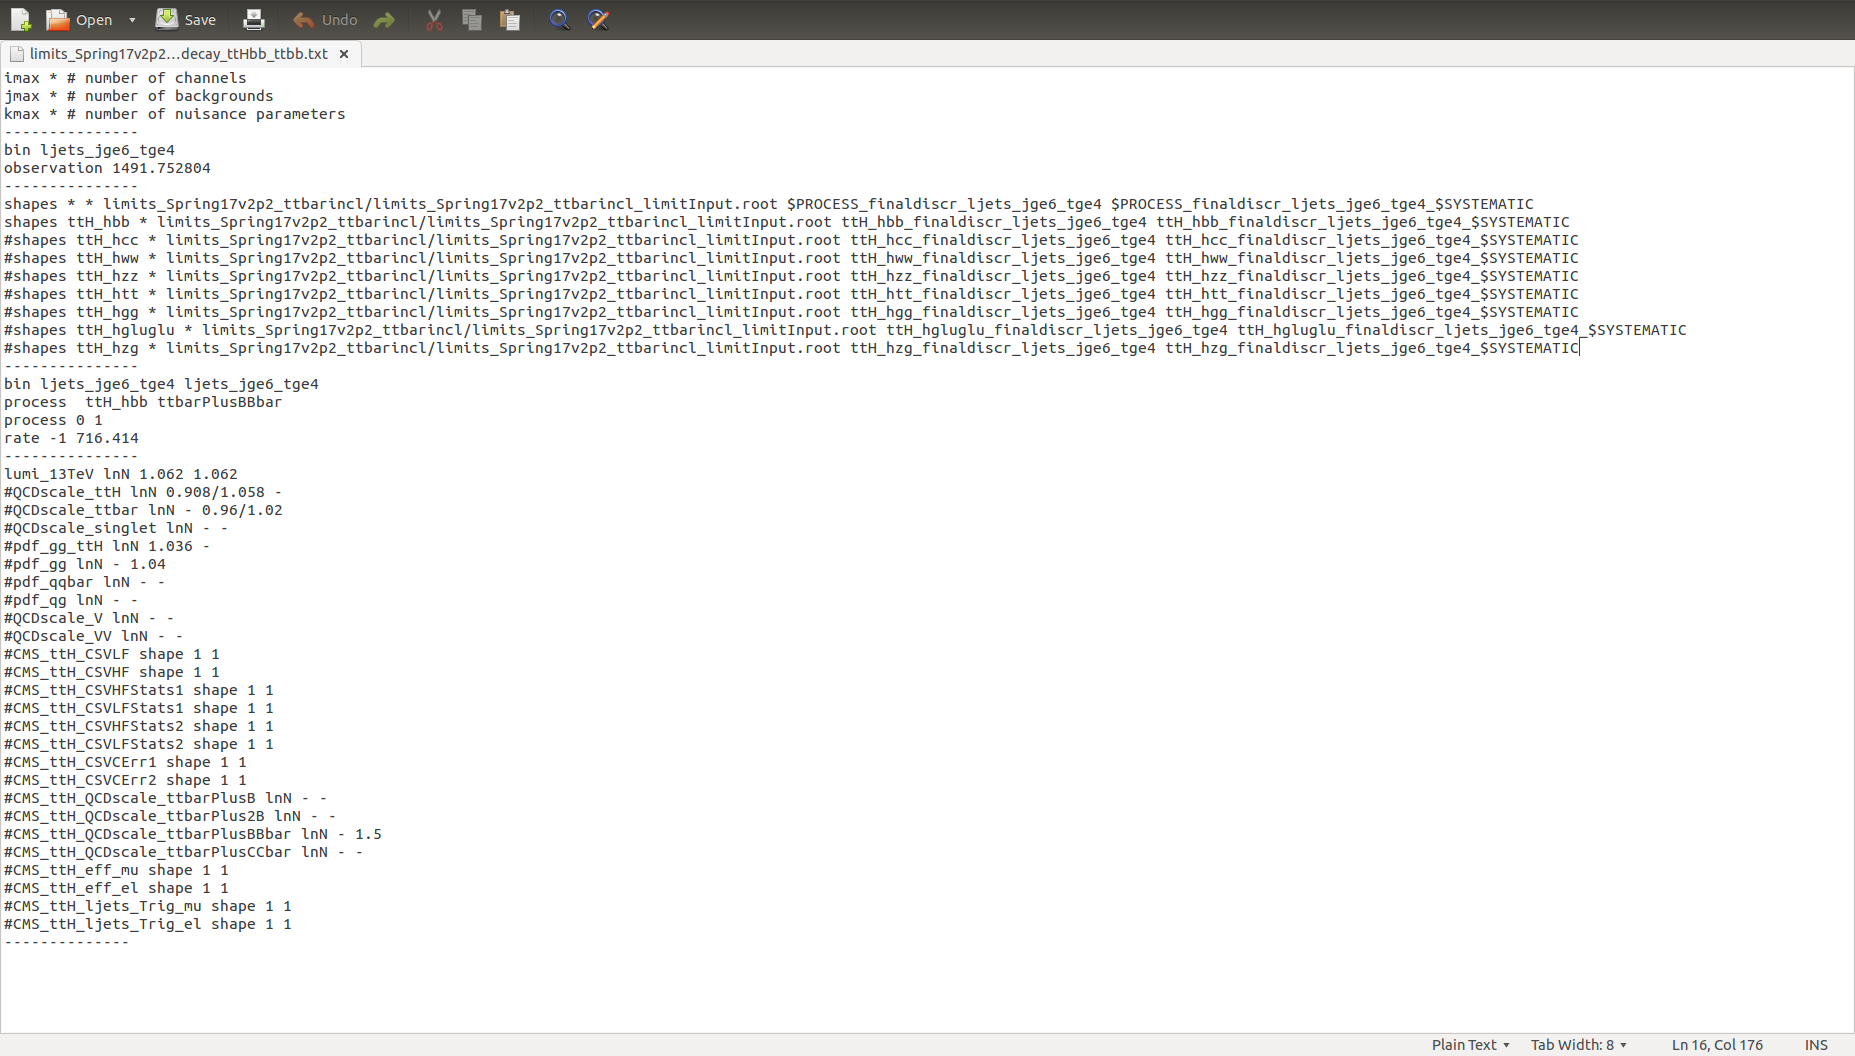
\includegraphics[width = \textwidth]{datacard.png}

\end{frame}



\begin{frame}{List of Processes}
\lstinputlisting[numbers=none, basicstyle=\tiny,  frame=none]{listOfProcesses.txt}
\end{frame}

\begin{frame}{List of Nuisance Parameters}
\lstinputlisting[numbers=none, basicstyle=\tiny,  frame=none]{listOfNP.txt}
\end{frame}

\begin{frame}{Mean Plots for jge6, tge4, lumiOnly}

\begin{figure}
\centering
\subfloat[$\mu = 0$]{\includegraphics[scale = 0.25]{plots/jge6_tge4_sig0_N1000_lumiOnly_POImeans.pdf}} $\qquad$
\subfloat[$\mu = 1$]{\includegraphics[scale = 0.25]{plots/jge6_tge4_sig1_N1000_lumiOnly_POImeans.pdf}}
\scriptsize\caption[jge6$\_$tge4$\_$N1000$\_$lumiOnly]{Mean Plots for jge6, tge4, only lumi Nuisance Parameter with 1000 Pseudo Experiments}
\end{figure}

\end{frame}

\begin{frame}{Mean Plots for jge6, tge4, allNP}

\begin{figure}
\centering
\subfloat[$\mu = 0$]{\includegraphics[scale = 0.25]{plots/jge6_tge4_sig0_N1000_allNP_POImeans.pdf}} $\qquad$
\subfloat[$\mu = 1$]{\includegraphics[scale = 0.25]{plots/jge6_tge4_sig1_N1000_allNP_POImeans.pdf}}
\scriptsize\caption[jge6$\_$tge4$\_$N1000$\_$allNP]{Mean Plots for jge6, tge4, all Nuisance Parameters with 1000 Pseudo Experiments}
\end{figure}

\end{frame}

\begin{frame}{Mean Plots for jge6, tge4, only \ttbarH\bbbar + \ttbar lf, lumiOnly}

\begin{figure}
\centering
\subfloat[$\mu = 0$]{\includegraphics[scale = 0.25]{plots/jge6_tge4_ttHbb_ttlf_N100_sig0_lumiOnly_POImeans.pdf}} $\qquad$
\subfloat[$\mu = 1$]{\includegraphics[scale = 0.25]{plots/jge6_tge4_ttHbb_ttlf_N100_sig1_lumiOnly_POImeans.pdf}}
\scriptsize\caption[jge6$\_$tge4$\_$ttHbb$\_$ttlf$\_$lumiOnly]{Mean Plots for jge6, tge4, only \ttbarH\bbbar + \ttbar lf, only lumi Nuisance Parameter with 100 Pseudo Experiments}
\end{figure}

\end{frame}

\begin{frame}{Mean Plots for jge6, tge4, only \ttbarH\bbbar + \ttbar \bbbar, lumiOnly}

\begin{figure}
\centering
\subfloat[$\mu = 0$]{\includegraphics[scale = 0.25]{plots/jge6_tge4_ttHbb_ttbb_N100_sig0_lumiOnly_POImeans.pdf}} $\qquad$
\subfloat[$\mu = 1$]{\includegraphics[scale = 0.25]{plots/jge6_tge4_ttHbb_ttbb_N100_sig1_lumiOnly_POImeans.pdf}}
\scriptsize\caption[jge6$\_$tge4$\_$ttHbb$\_$ttbb$\_$lumiOnly]{Mean Plots for jge6, tge4, only \ttbarH\bbbar + \ttbar \bbbar, only lumi Nuisance Parameter with 100 Pseudo Experiments}
\end{figure}

\end{frame}

\begin{frame}{Mean Plots for jge6, t3, lumiOnly}

\begin{figure}
\centering
\subfloat[$\mu = 0$]{\includegraphics[scale = 0.25]{plots/jge6_t3_sig0_N1000_lumiOnly_POImeans.pdf}} $\qquad$
\subfloat[$\mu = 1$]{\includegraphics[scale = 0.25]{plots/jge6_t3_sig1_N1000_lumiOnly_POImeans.pdf}}
\scriptsize\caption[jge6$\_$t3$\_$lumiOnly]{Mean Plots for jge6, t3, only lumi Nuisance Parameter with 1000 Pseudo Experiments}
\end{figure}

\end{frame}

\begin{frame}{Mean Plots for jge6, t3, allNP}

\begin{figure}
\centering
\subfloat[$\mu = 0$]{\includegraphics[scale = 0.25]{plots/jge6_t3_sig0_N1000_allNP_POImeans.pdf}} $\qquad$
\subfloat[$\mu = 1$]{\includegraphics[scale = 0.25]{plots/jge6_t3_sig1_N1000_allNP_POImeans.pdf}}
\scriptsize\caption[jge6$\_$t3$\_$allNP]{Mean Plots for jge6, t3, all Nuisance Parameter with 1000 Pseudo Experiments}
\end{figure}

\end{frame}

\begin{frame}{$\mu$ Distribution Plots for higher luminosity}

\begin{figure}
\centering
\subfloat[$\mu = 0$]{\includegraphics[scale = 0.25]{plots/jge6_tge4_ttHbb_ttbb_scaledBy12900_sig0_N100_lumiOnly_decorrelated_POI.pdf}} $\qquad$
\subfloat[$\mu = 1$]{\includegraphics[scale = 0.25]{plots/jge6_tge4_ttHbb_ttbb_scaledBy12900_sig1_N100_lumiOnly_decorrelated_POI.pdf}}
\scriptsize\caption[jge6$\_$tge4$\_$tthbb\_ttbb\_lumiOnly\_highLumi]{jge6$\_$tge4$\_$tthbb\_ttbb\_lumiOnly\_highLumi, 100 Pseudo Experiments}
\end{figure}

\end{frame}

% PUT BACKUP SLIDES HERE

%%%

\backupend
\end{document}





